\documentclass{article}
\usepackage{graphicx} % Required for inserting images

\usepackage[UTF8]{ctex}
\usepackage{setspace}
\usepackage{listings}
\usepackage{xcolor}
\usepackage{listings}
\usepackage[colorlinks,linkcolor=blue]{hyperref}

\lstset{
  backgroundcolor=\color{white},
  basicstyle=\ttfamily\footnotesize,
  breakatwhitespace=false,
  breaklines=true,
  captionpos=b,
  commentstyle=\color{mygreen},
  deletekeywords={...},
  escapeinside={\%*}{*)},
  frame=single,
  keepspaces=true,
  keywordstyle=\color{blue},
  language=Python,
  morekeywords={*,...},
  numbers=left,
  numbersep=5pt,
  numberstyle=\tiny\color{mygray},
  rulecolor=\color{black},
  showspaces=false,
  showstringspaces=false,
  showtabs=false,
  stepnumber=2,
  stringstyle=\color{mymauve},
  tabsize=2,
  title=\lstname
}


% Set page size and margins
% Replace `letterpaper' with `a4paper' for UK/EU standard size
\usepackage[letterpaper,top=2cm,bottom=2cm,left=3cm,right=3cm,marginparwidth=1.75cm]{geometry}

% Useful packages
\usepackage{amsmath}
\usepackage{graphicx}
\usepackage[colorlinks=true, allcolors=blue]{hyperref}

\title{数据挖掘期末项目}
\author{温兆和 10205501432}

\begin{document}

\maketitle

\section{项目背景}
由于客户的流失会给企业带来巨大的损失,我们需要根据用户过往的消费数据预测其流失的可能性,以挽回客户并减少挽回工作的工作量。在本次课程项目中,我们考虑一个给商户提供服务的应用平台。该应用平台上有许多商户,商户下面又有一个或者多个店铺。如果一个店铺在某一天前的五天(包括那一天在内)之内,前三天有⼤于二元的交易,后两天⽆交易,就认为该店铺被其所有者抛出;如果某个店铺在抛出后二十八天中没有交易,就认为该店铺流失。我们需要做的,就是从该平台所有商户的流水数据、商户数据以及借贷记录中提取出抛出店铺的相关数据,并训练一个模型,预测抛出的店铺是否会流失。

\section{数据预处理}
本项目中,我所做的数据预处理并不算多。首先,我删除了各个数据集中完全重复的数据。然后,我统计了所有数据表中的缺失值,发现整个数据集中只有流水数据的\lstinline{paid_amount}字段有缺失情况。

\begin{figure}[h]
    \centering
    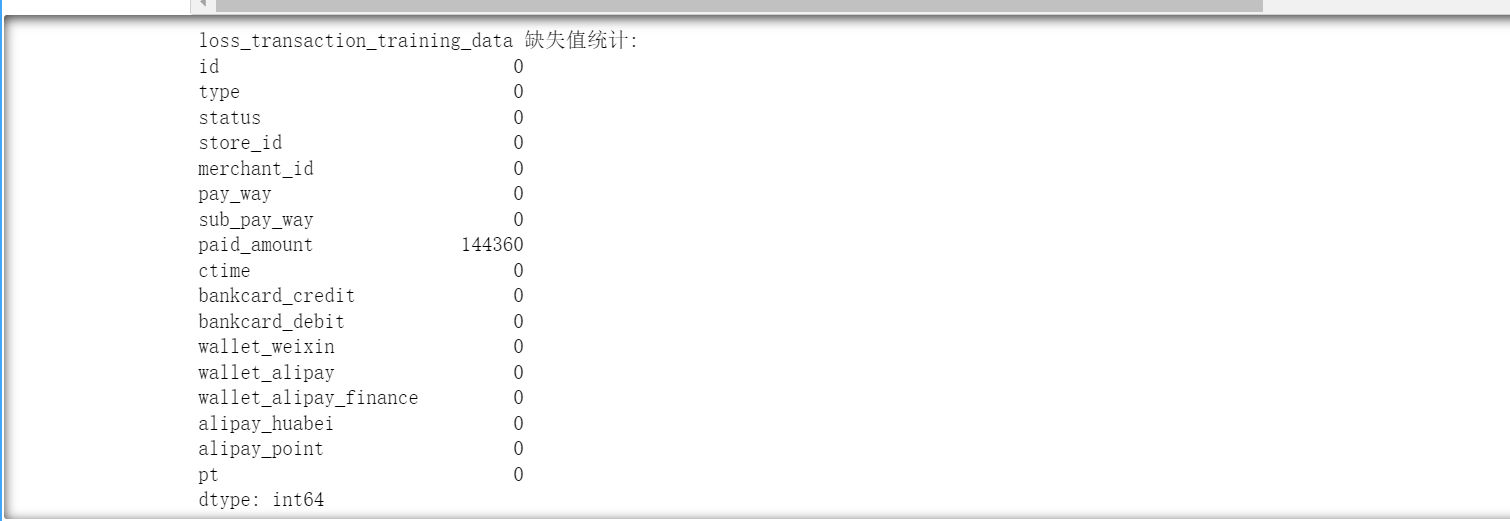
\includegraphics[width=0.75\linewidth]{img/image01.png}
    \caption{数据集缺失值统计结果(流水部分)}
    \label{fig:enter-label}
\end{figure}

因为\lstinline{paid_amount}很容易就能从流水数据的\lstinline{bankcard_credit}、\lstinline{bankcard_debit}、\lstinline{wallet_weixin}、\lstinline{wallet_alipay}、\lstinline{wallet_alipay_finance}、\lstinline{alipay_huabei}和\lstinline{alipay_point}计算出来,所以我直接用缺失数据各种支付方式支付金额之和填补其\lstinline{paid_amount}字段。

\begin{lstlisting}
# 定义函数计算 paid_amount
def calculate_paid_amount(row):
    paid_amount = row['bankcard_credit'] + row['bankcard_debit'] + row['wallet_weixin'] + row['wallet_alipay'] + row['wallet_alipay_finance'] + row['alipay_huabei'] + row['alipay_point']
    return paid_amount
\end{lstlisting}

最后,我从训练集中删除了所有不符合抛出条件的数据。在整个抛出点数据训练集中,有$805$条数据不符合“前三天有⼤于二元的交易”,有$40$条数据不符合“后两天⽆交易”,总共删去了$842$条不符合抛出条件的错误数据。

\begin{figure}[h]
    \centering
    
\includegraphics[width=0.75\linewidth]{img/image02.png}
    \caption{抛出数据正确性检查结果}
    \label{fig:enter-label}
\end{figure}

此外,部分数据交易总金额的值与各支付方式交易金额之和不等。对于交易总金额大于各支付方式交易金额之和的情况,把交易总金额多出的部分作为“红包支付”的金额;对于交易总金额大于各支付方式交易金额之和的情况,把交易总金额修改为各支付方式交易金额之和。

\section{特征提取}
在进行数据预处理后,我提取了以下特征:

\begin{itemize}
    \item \lstinline{industry_level1}:该商户所在的行业
    \item \lstinline{province}:该商户所在省份
    \item \lstinline{max_pay_way}:该商户顾客首要支付方式
    \item \lstinline{max_sub_pay_way}:该商户顾客次要支付方式
    \item \lstinline{past_mon_lend_amount}:抛出前一个月内商户贷款总额
    \item \lstinline{past_mon_lend_period}:抛出前一个月内商户贷款期数
    \item \lstinline{past_mon_overdue}:抛出前一个月内商户逾期还款次数
    \item \lstinline{avg_paid_amount}:该商户所有成功交易的总金额平均值
    \item \lstinline{avg_bankcard_credit}:该商户所有成功交易的信用卡支付金额平均值
    \item \lstinline{avg_bankcard_debit}:该商户所有成功交易的储蓄卡支付金额平均值
    \item \lstinline{avg_wallet_weixin}:该商户所有成功交易的微信余额支付金额平均值
    \item \lstinline{avg_wallet_alipay}:该商户所有成功交易的支付宝支付金额平均值
    \item \lstinline{avg_wallet_alipay_finance}:该商户所有成功交易的余额包支付金额平均值
    \item \lstinline{avg_alipay_huabei}:该商户所有成功交易的花呗支付金额平均值
    \item \lstinline{avg_alipay_point}:该商户所有成功交易的集分宝金额平均值
    \item \lstinline{avg_red_envp_pay}:该商户所有成功交易的红包支付金额平均值
    \item \lstinline{type_percentage}:该商户交易类型为“取消”或“退款”的交易占比
    \item \lstinline{status_percentage}:该商户不成功交易的占比
\end{itemize}

经过老师的指导,我又添加了以下特征:

\begin{itemize}
    \item \lstinline{store_id_count}:该商户旗下所有门店的总数量, 反映了商户规模
    \item \lstinline{high_credit_days}:抛出前一个月内商户高额借贷天数
    \item \lstinline{high_credit_transaction_count}:抛出前一个月内商户高额借贷笔数
    \item \lstinline{no_transaction_ratio}:抛出前一个月内无交易日天数占比
    \item \lstinline{credit_card_payment_ratio}:抛出前一个月内信用卡交易金额占比,因为信用卡类似于一种形式的“赊账”,顾客不还会导致商户损失
    \item \lstinline{integer_10_transactions}:抛出前一个月内交易金额为十的整数倍的交易笔数,这可能是刷单刷出来的
\end{itemize}
在提取完特征后,我对每个特征进行了卡方检验,来检验这些特征是否对响应变量(也就是店铺是否流失)有显著作用。经过检验,\lstinline{wallet_alipay_finance}、\lstinline{type_percentage}、\lstinline{high_credit_days}和\lstinline{high_credit_transaction_count}对响应变量效果不显著,所以直接删去。删掉不显著的特征有助于减少过拟合、提高模型的泛化能力。之后,检查训练集中是否存在多重共线性。多重共线性会导致训练出的回归系数不稳定,进而影响模型的预测能力。在画出的seaborn热力图中,除对角线外绝大部分的格点颜色较深,说明数据集中不存在严重的多重共线性现象。

\begin{figure}[h]
    \centering
    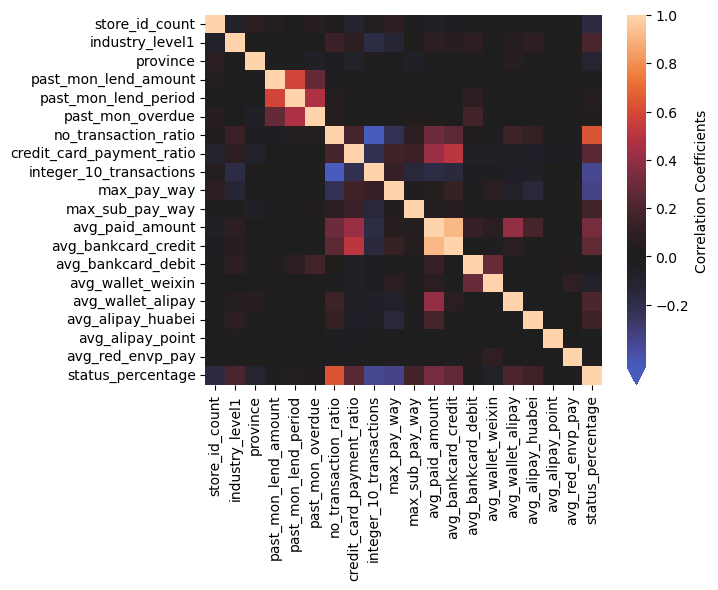
\includegraphics[width=0.75\linewidth]{img/image03.png}
    \caption{多重共线性检测结果:seaborn热力图}
    \label{fig:enter-label}
\end{figure}

\section{模型选择与训练}
至此,我们已经得到了可以直接输入模型的训练数据,接下来只要训练模型即可。首先,我选择了逻辑斯蒂回归、支持向量机、决策树、感知机和随机森林这五种最基础的机器学习分类模型,将既有的训练集按照$8:2$的比例划分为训练集和验证集,用训练集训练模型并在验证集上检测模型的准确率。得到的结果如下所示:

\begin{figure}[h]
    \centering
    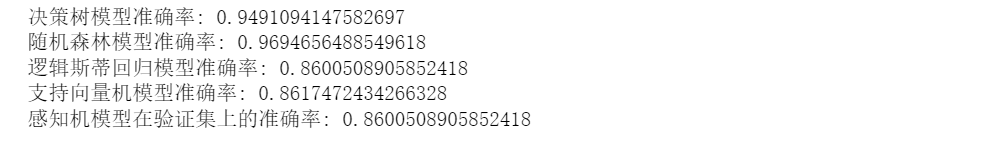
\includegraphics[width=0.75\linewidth]{img/image04.png}
    \caption{五种模型在验证集上的准确率}
    \label{fig:enter-label}
\end{figure}

其中,随机森林的准确率最高,决策树次之,另外三种模型则稍低一些。

我们再对刚才训练得到的随机森林模型进行五折交叉验证:
\begin{figure}[h]
    \centering
    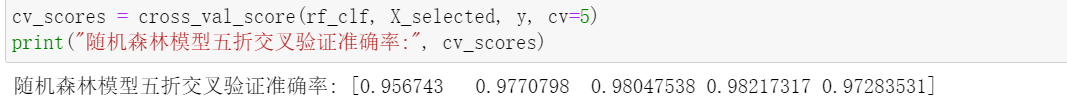
\includegraphics[width=0.75\linewidth]{img/image05.png}
    \caption{随机森林五折交叉验证}
    \label{fig:enter-label}
\end{figure}

可以看出,随机森林在这个数据集上的性能是相当好的。

\section{结果分析与总结}
首先,分析一下为什么决策树的性能会好过其他分类器,随机森林的性能又好于决策树。除了数据集本身的非线性和复杂性之外,决策树本身有一个特点,就是它是对各个特征分别进行分类的,而不是把特征的值代进去算,而且一个特征越重要(在决策树中是信息熵高),决策树就越先对它进行分类。显然,决策树考虑了特征的重要程度,而且我们使用的数据集中本身就包含了“商户所属行业门类”和“商户所在省份”这些分类变量,里面的$1$、$2$……都是指代一个省份或者一个行业门类的,在模型中对它进行算数运算显然是不适合的,而决策树就没有这个问题。而随机森林可以通过集成多个决策树的预测结果来减少过拟合并提高模型的泛化能力。

其次,再谈谈自己对本次课程项目的感想。在学习《数据挖掘》课程之前,我一直以为“数据智能”问题中,最关键的部分是模型的选择和性能分析,但做完这个项目后,我意识到其实更重要的是数据预处理和特征选择。从删除重复值、填补缺失值到检查抛出点数据的正确性,我花费了大量的时间精力编写代码、向助教和老师咨询沟通,因为这直接关乎到模型的性能,甚至是我们所做的工作是否有意义。而经过处理的原始数据集是无法直接用于训练模型的,我们必须从中自行提取特征。刚开始我绞尽脑汁想出了不少可能和商户是否流失有关的特征,但通过老师的指导,我发现还是有一些被我忽略的可能与是否流失相关的特征。比如说“整十金额交易比重”,我自己原先根本不可能想到这一点,但是经过老师的指导,我意识到整十交易可能是在刷单,这能反映出商户的经营状态是否正常。卡方检验的结果也证明这一特征对响应变量的作用是显著的。而《数据挖掘》这门课本身就是教我们如何从数据中发掘出我们不容易意识到的事物间的潜在关联,这也是我们在今后继续学习和感悟的。事实也证明,只要做好了数据处理和特征提取,哪怕用的是最简单的模型,准确率也没有低于$85\%$的。

\end{document}
